% !TeX spellcheck = en_GB
% !TeX root = ../main-scirep.tex

\begin{figure}[H]
	\centering
		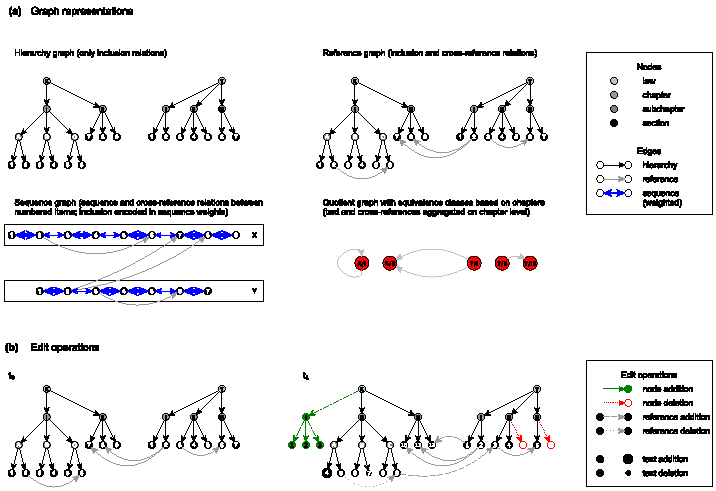
\includegraphics[width=\textwidth]{{figures/figure1}}
	\caption{Dynamic network data model for legislative document collections. All figures created by the authors.}
	\label{fig:conceptual_sequence_graph}
\end{figure}

% Data updated: 2020-07-28 
\begin{table}[H]
	\centering
	\footnotesize
	\bgroup
	\def\arraystretch{1.5}
	\begin{tabular}{L{0.1\linewidth}R{0.1\linewidth}R{0.1\linewidth}R{0.1\linewidth}R{0.05\linewidth}R{0.1\linewidth}R{0.1\linewidth}R{0.1\linewidth}}
		&\multicolumn{3}{c}{\textbf{United States}}&&\multicolumn{3}{c}{\textbf{Germany}}\\
		&\textbf{1994}&\hfill\textbf{2018}\hfill&$\Delta$&&\hfill\textbf{1994}\hfill&\hfill\textbf{2018}\hfill&$\Delta$\\\hline
		\textbf{Tokens}
		% US
		& $14.0$~M%14005682
		& $21.2$~M%21153109
		& $51~\%$%Ratio: 1.5103233816104065
		&
		% DE
		& $4.5$~M%4521580
		& $7.4$~M%7433500
		& $64~\%$%Ratio: 1.6440049717134275
		\\\hline
		\textbf{Structures} % this is ALL structures, including subseqitems. 
		% US
		&$452.4$~K%452370
		&$828.1$~K%828089
		&$83~\%$%Ratio: 1.8305568450604595
		&
		% DE
		&$120.6$~K%120683
		&$161.4$~K%161446
		&$34~\%$%Ratio: 1.3377691969871481
		\\\hline
		\textbf{References}
		% US
		&$58.0$~K%58007
		&$88.6$~K%88646
		&$53~\%$%Ratio: 1.528194873032565
		&
		% DE
		&$76.9$~K%76876
		&$139.1$~K%139147
		&$81~\%$%1.8100187314636558
	\end{tabular}
	\egroup\caption{Federal legislation in the United States and Germany: descriptive statistics ($1994$ and $2018$).}\label{tab:descriptive-statistics}
\end{table}


\clearpage

\begin{figure}[H]
	\centering
	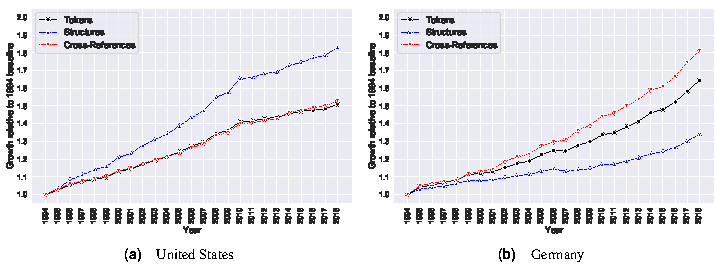
\includegraphics[width=\textwidth]{{figures/figure2}}
	\caption{Federal legislation in the United States and Germany: growth statistics  (1994--2018).}
	\label{fig:legislative-growth}
\end{figure}

\begin{figure}[H]
	\centering
	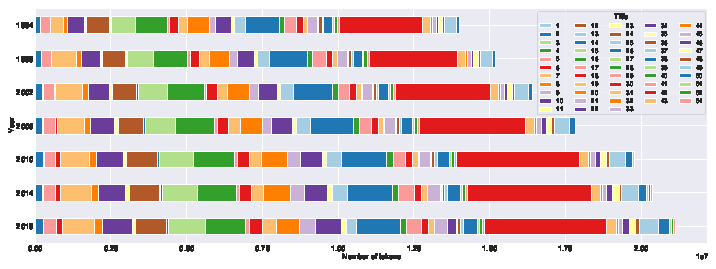
\includegraphics[width=\textwidth]{{figures/figure3}}
	\caption{Federal legislation in the United States by Title (1994--2018), measured in tokens.}
	\label{fig:us-tokens-per-title}
\end{figure}

\newpage

\begin{figure}[H]
	\vspace*{-40pt}
	\centering
	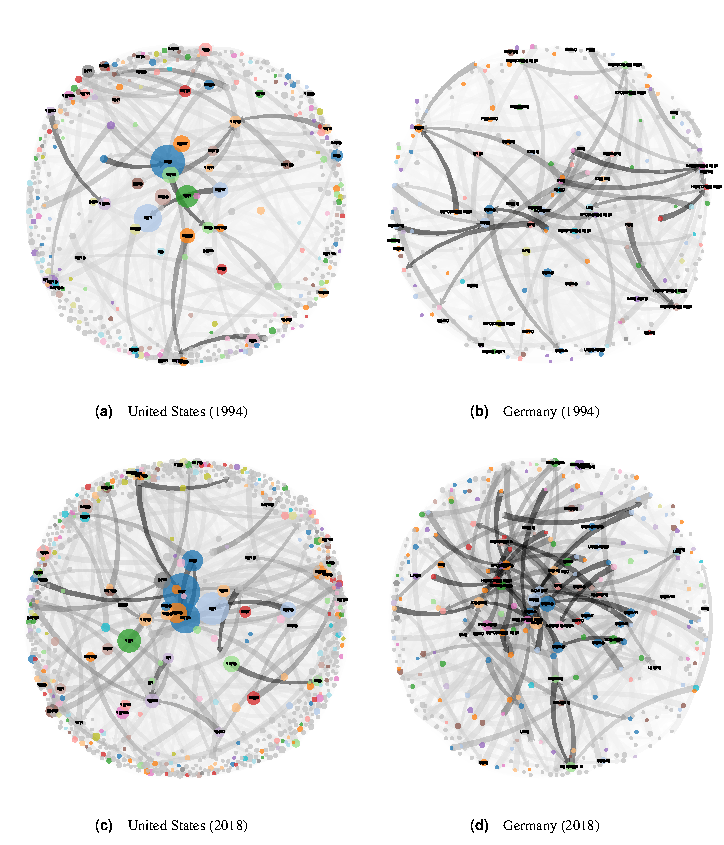
\includegraphics[width=\textwidth]{{figures/figure4}}
	\caption{Federal legislation in the United States and Germany: quotient graphs by Title/Chapter (United States) and Law Name/Book (Germany) (1994 and 2018),
		with arrows running between nodes indicating that text contained in one node cites text contained in another node.
		Node sizes indicate token counts (larger $=$ more tokens), where only nodes with at least $5000$ tokens (corresponding to roughly ten pages) are shown.
		For each nation separately, nodes share the same colour if they are placed in the same cluster family,
		and nodes not in one of the $20$ largest cluster families are coloured in grey.
		Only the labels of the 50 largest nodes (measured in tokens) are drawn.
	}
	\label{fig:us-de-chapter-quotient}
\end{figure}

%\clearpage

\begin{figure}[H]
	\centering
	\vspace*{-16pt}
	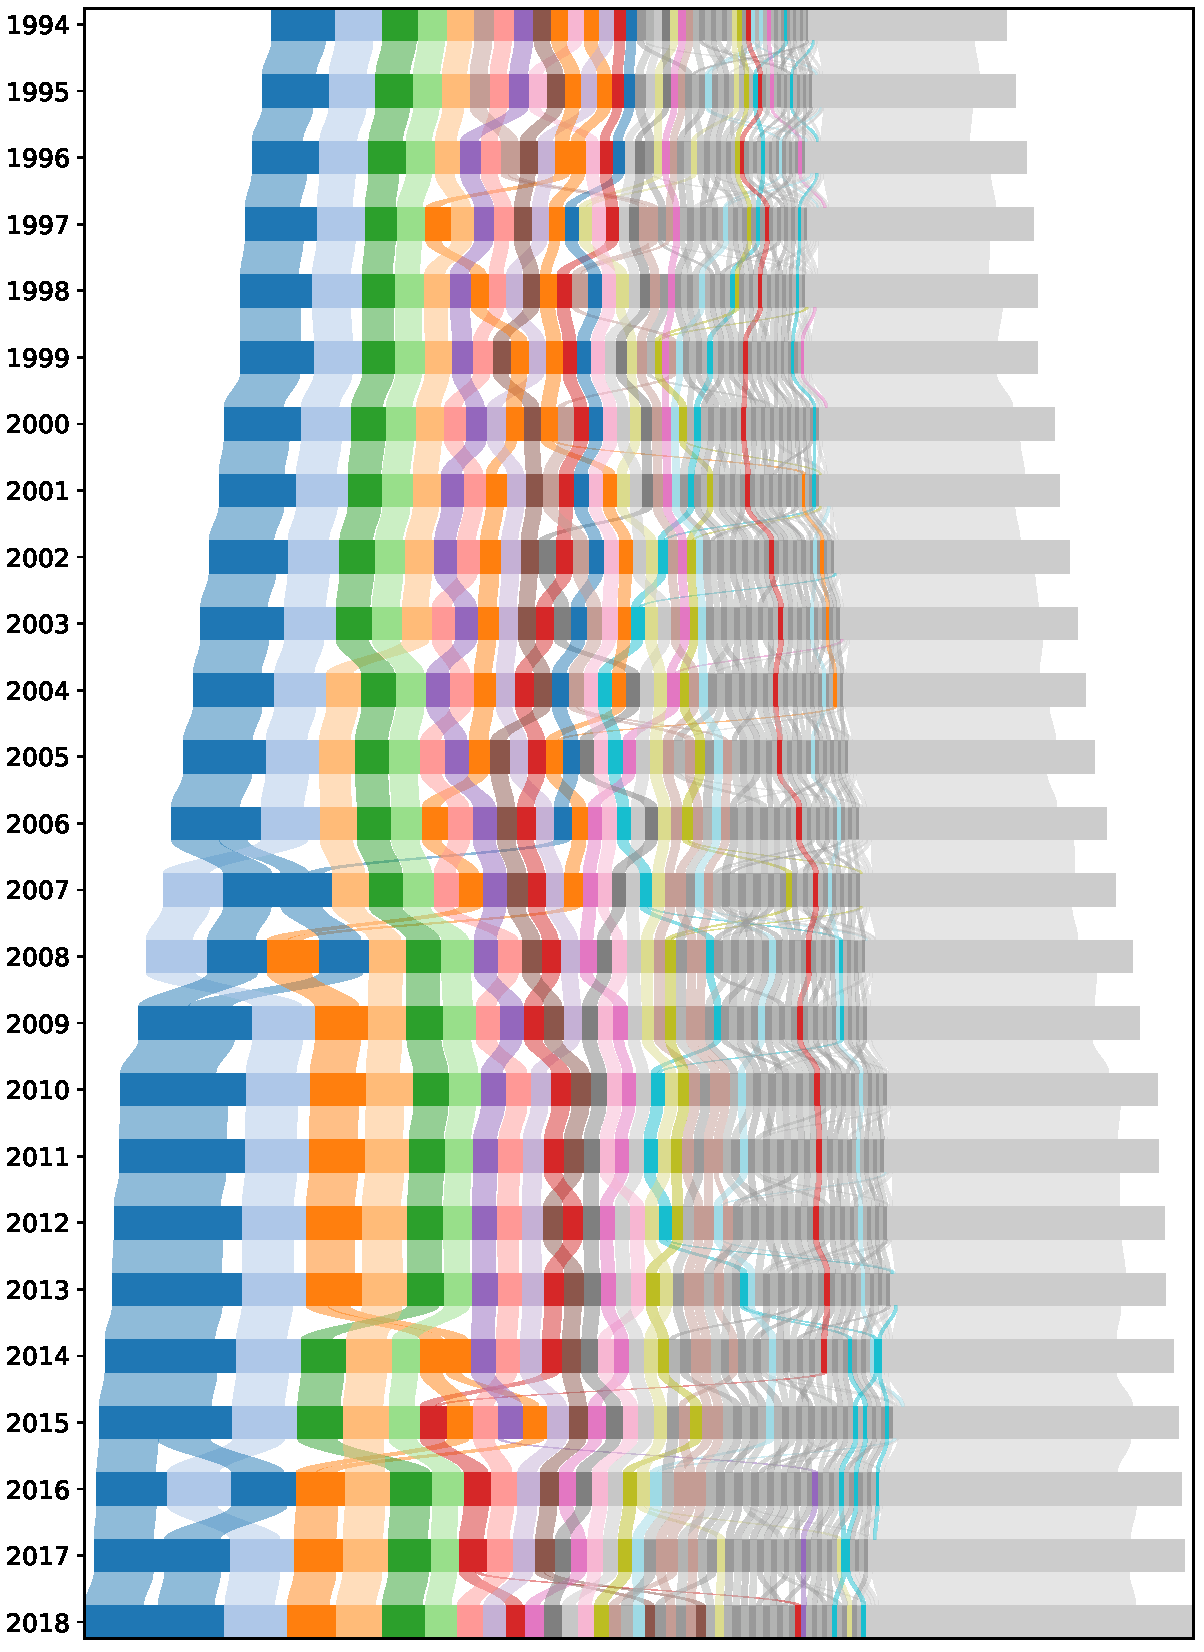
\includegraphics[width=0.9\textwidth]{{figures/figure5}}
	\caption{%
		Federal legislation in the United States by cluster (1994--2018). 
		Each block in each year represents a cluster. 
		Clusters are ordered from left to right by decreasing size (measured in tokens) and coloured by the cluster family to which they belong, 
		where clusters not in one of the $20$ largest cluster families are coloured in alternating greys. 
		Small clusters are summarised in one miscellaneous cluster, which is always the rightmost cluster and coloured in light grey.
		A full legend mapping colours to legal topics can be found in Section 5.1 of the~\suppi.
	}
	\label{fig:sankey}
\end{figure}

\clearpage

\begin{figure}[H]
	\centering
	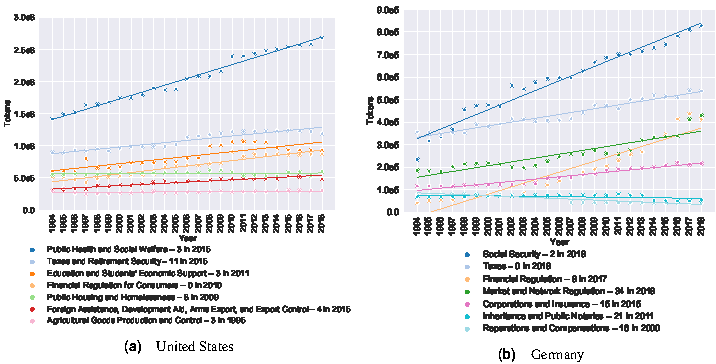
\includegraphics[width=\textwidth]{{figures/figure6}}
	\caption{Federal legislation in the United States and Germany: growth statistics by cluster family for selected cluster families (1994--2018).
	The legends are sorted by the $y$-values of the regression lines in $2018$.
	The colours are comparable across countries, i.e., \emph{same colour} $\Leftrightarrow$ \emph{(roughly) same topic}.
	}
	\label{fig:legislative-growth-cluster}
\end{figure}
